\documentclass{article}
\usepackage[utf8]{inputenc}
\usepackage{amsmath}
\newcommand{\dd}[1]{\mathrm{d}#1}
\usepackage{url}
\renewcommand{\refname}{Referencias}
\usepackage{float}

\title{Redes Neuronales \\
  \large Práctico 3 \\
  }
\author{Mariano Politano }
\date{Noviembre 2020}

\usepackage{natbib}
\usepackage{graphicx}

\begin{document}

\maketitle




En el presente práctico, trabajamos con un  \textbf{autoencoder} que es una red neuronal feed-forward. Utilizamos el conjunto de datos MNIST.

A diferencia de un aprendizaje supervisado, donde se intenta predecir algo sobre la entrada, un \textbf{autoencoder} se utiliza para aprender una representación distribuida de nuestros datos de entrenamiento e incluso se puede utilizar para generar nuevas instancias de los datos de entrenamiento. 
En nuestro caso se utilizó para aprender la función identidad con la base de datos MNIST de dígitos escritos a mano y digitalizados.
Las imagenes tiene un tamaño de 28 x 28 pixeles en escalad de grises con 256 valores de intesidad.
En la \ref{fig1} se puede ver algunos ejemplos del dataset.
\begin{figure}[H]
\centering
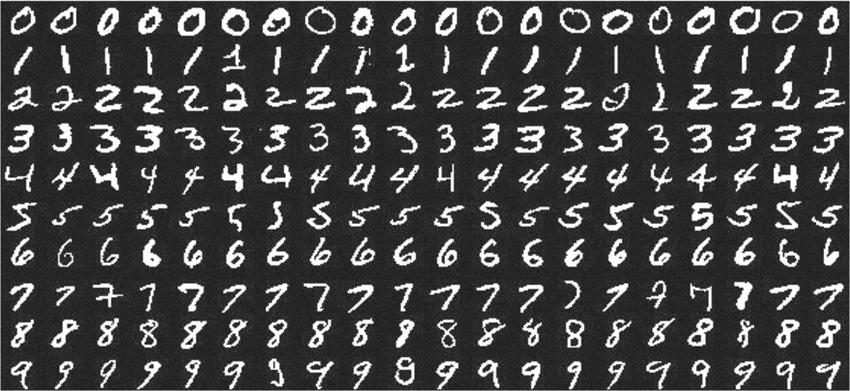
\includegraphics[width=\textwidth]{example.png}
\caption{Dataset de MNIST.}
\label{fig1}
\end{figure}



Un modelo \textit{feed-forward autoencoder} contiene dos componentes:

\begin{itemize}
\item Un codificador que toma una imagen como entrada y genera una representación de baja dimensión de la imagen.
\item Un decodificador que toma la incrustación de baja dimensión y reconstruye la imagen. 
\end{itemize}






los datos de  para el potencial de membrana de una neurona. Este modelo se comporta similar a cuando se le inyecta una corriente externa a un capacitador en paralelo con una resistencia.  Las neuronas mantienen una diferencia de potencial en su interior respecto del exterior y de acuerdo a lo  visto en clases sobre lo propuesto por \textbf{\textit{Lapicque}} en 1907 lo podemos  modelar  por la siguiente ecuación:
\begin{equation}
\label{eq1}
\frac{\partial V_{m}(t)}{\partial t} = \frac{1}{\tau_{m}}(E_{L} - V_{m}(t) + R_{m}I_{e}(t)).
\end{equation}
\

Donde $E_{L}$ es el potencial en reposo, $I_{e}(t)$ es una corriente eléctrica externa que se inyecta, $R_{m}$ es la resistencia y $\tau_{m}$ es el tiempo característico de la membrana $τm = r_{m} c_{m}$ (donde  $r_{m}$ y  $c_{m}$ son respectivamente la resistencia y la capacitancia de la membrana por unidad de área).

\

La ecuación \ref{eq1} del modelo  es una ecuación diferencial de primer orden, con una sola incógnita que es V. Tomando a  \textit{$I_{e}$} independiente del tiempo, por ende, es constante, y sin umbral de disparo, se  llega a la siguiente \textbf{resolución analítica}:
\begin{equation}
\notag

U(t) = V_{m}(t) - E_{L} - R_{m}               \rightarrow 
      \frac{\partial V_{m}(t)}{\partial t} = \frac{\partial U(t)}{\partial t}
\label{eq2}
\end{equation}
\begin{equation}
\notag
\frac{\partial U(t)}{\partial t} = -\frac{U(t)}{\partial t}      \rightarrow 
     U(t) = U_{o}e^{-\frac{t}{\tau_{m}}}
\end{equation}

Luego de esto, reemplazando, se puede llegar a la resolución:

\begin{equation}
V(t) = E_{L} + R_{m}I_{e} +(V(0) -  E_{L} - R_{m}I_{e})e^{-\frac{t }{\tau_{m}}}
\label{eq2}
\end{equation}

Tal como lo discutimos y analizamos en las clases, se puede observar que se arriba a la ecuación \ref{eq2}, con un simple cambio de variables. La neurona comienza con un potencial de membrana igual al potencial de reposo y se despolariza hasta alcanzar el valor  $E_{l} - R_{m}I_{e}$.

\
Como lo pedía el práctico, resolvemos está ecuación para el caso en que\textbf{ $I_{e}$ sea igual a 2 nA}. Los valores de los parámetros son:
$V_m(t = 0) = EL = −65 mV$, $R = 10 m\Omega$, $Vth = −50 mV$, $\tau_{m} = 10 ms$ y el paso de integración es $h = 0.05$.
Se utiliza el método Runge-Kutta de orden cuatro para encontrar una solución aproximada. La solución se muestra en el siguiente gráfico:




Se puede observar que cuando no hay disparo (linea azul), la función aumenta y llega a saturar al valor -45 que es $E_L + R_mI_e$. En cambio cuando hay disparo (linea naranja), al llegar al umbral ($-50$ mV) se resetea el voltaje y nunca se estabiliza. 

\section*{Frecuencia disparo}
En esta sección analizaré cada cuanto tiempo dispara una neurona. Modifique el algoritmo para contar la cantidad de veces que dispara en el intervalo de tiempo (0-200) para diferentes valores de corrientes (de 0 a 6 nA).

\begin{figure}[H]
\centering
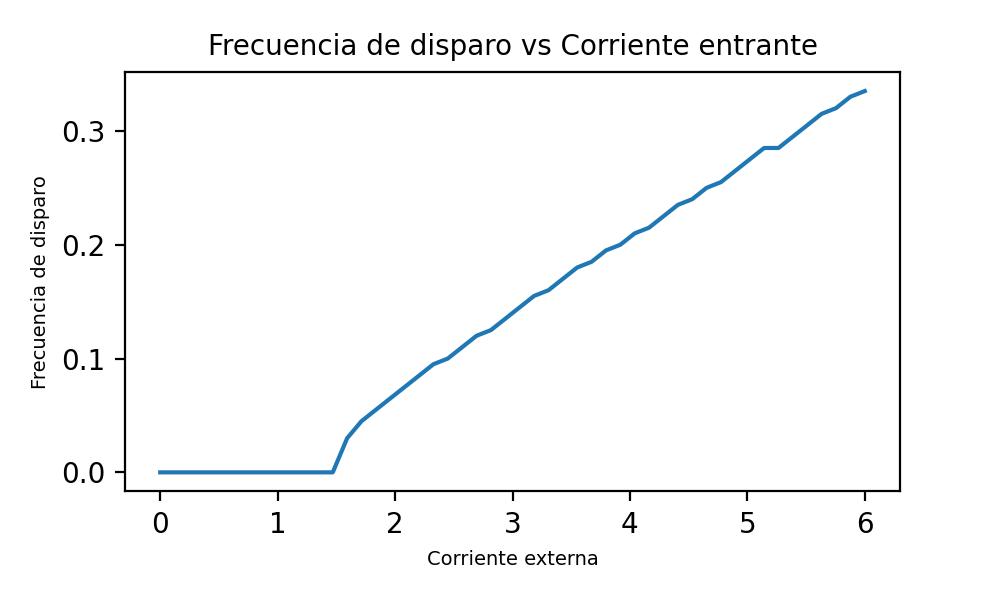
\includegraphics[width=\textwidth]{frecvscorri.png}
\caption{Frecuencia de disparo para diferentes corrientes.}
\label{frecuencia}
\end{figure}

 Como se puede observar, para corrientes muy bajas (menores a 1.5nA), la neurona no supera nunca el umbral. Sino que alcanza un potencial de menor valor y se mantiene constante en él. Esto se debe a que la corriente inyectada no es lo suficientemente intensa como para provocar un potencial de acción. Este comportamiento se puede ver mejor en los gráficos de la figura \ref{graficos}. Vale aclarar que, para dos corrientes puede existir la misma cantidad de disparos, pero con una leve diferencia de período. Ese comportamiento se observa en la variaciones de la "recta" en la figura \ref{frecuencia}.

Agrego los  gráficos con distintas corrientes en la figura \ref{graficos}. En ellos, se puede observar con mas claridad que con 1.5nA, la neurona no llega a disparar. Con una corriente 1.6nA se producen muy pocos disparos si se lo compara con una corriente de 4nA. 
Con esto se puede concluir que cuanto mayor es la corriente, mas disparos provoca.

\begin{figure}[H]
\centering
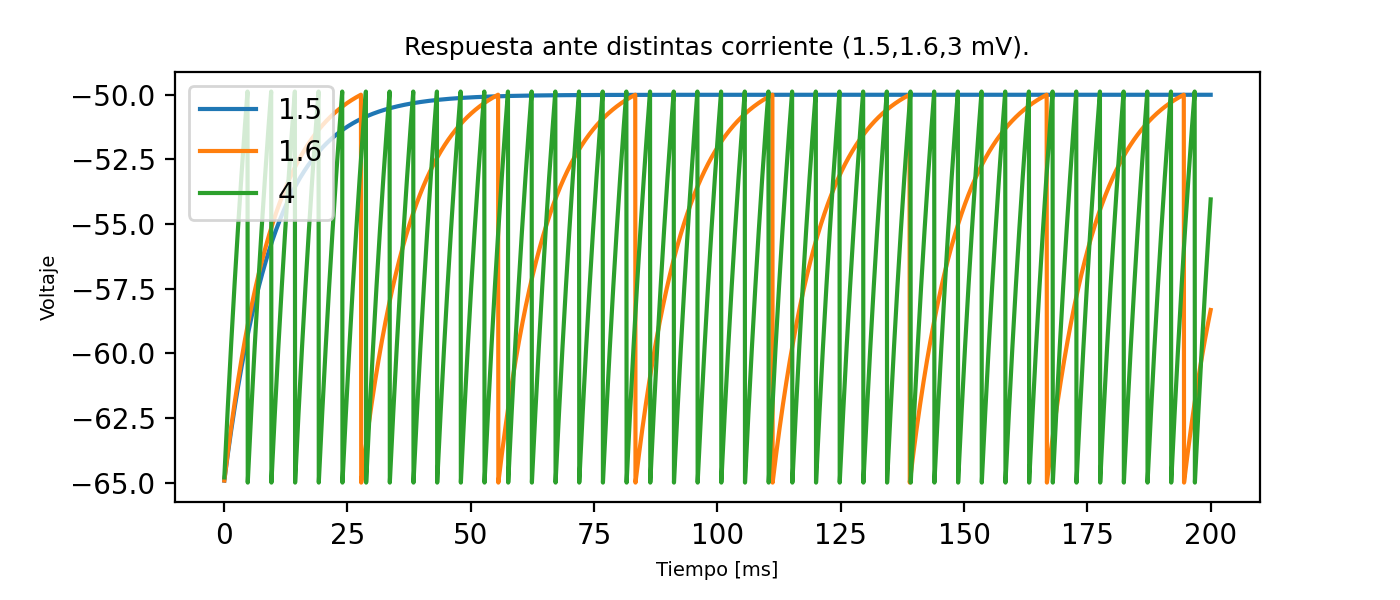
\includegraphics[width=\textwidth]{graficos.png}
\caption{Potencial de membrana para diferentes corrientes. }
\label{graficos}
\end{figure}


\section{Aleatoria}
Si ahora tomamos una corriente que no es constante, sino que elegimos una corriente aleatoria procedente de una distribución uniforme en el intervalo [0,5]nA. Obtenemos el siguiente gráfico.
 
\begin{figure}[H]
\centering
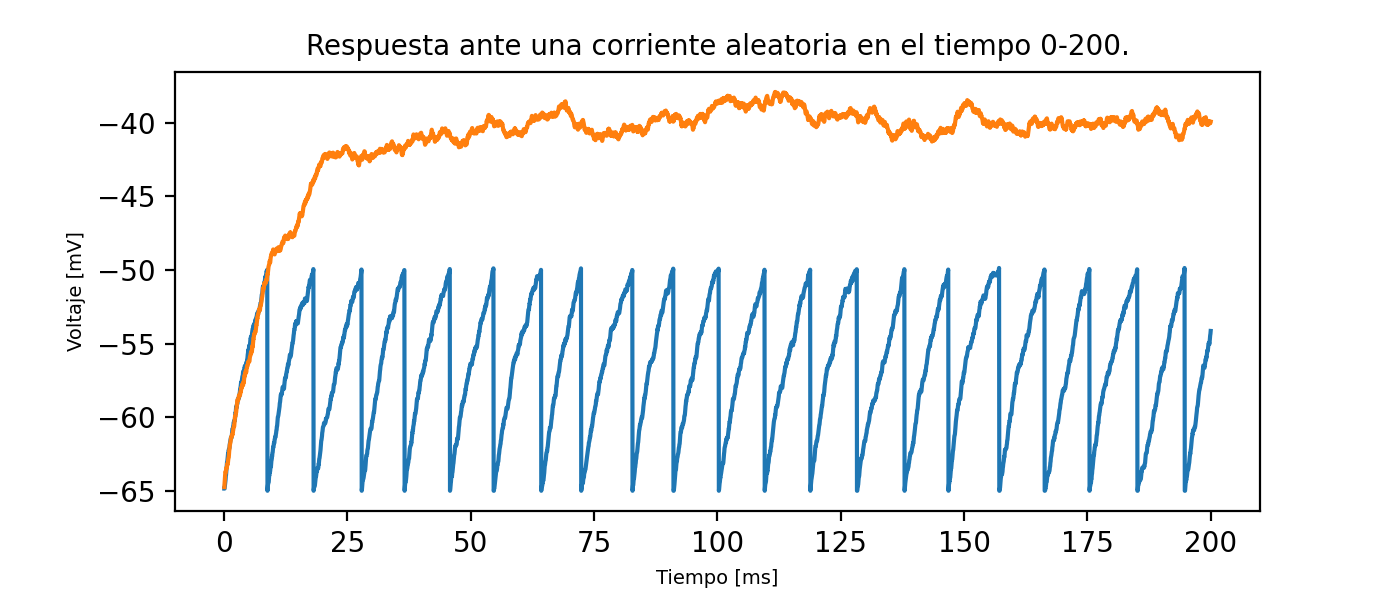
\includegraphics[width=\textwidth]{aleatorioConSin.png}
\caption{Potencial de membrana para corriente aleatoria entre 0-5nA. }
\label{aleatorio}
\end{figure}

Se puede ver que la linea naranja(sin disparo) crece exponencialmente, y luego se mueve de manera mas errática que con una corriente constante. Cuando agregamos el disparo (linea azul) se restablece cuando llega al umbral pero la frecuencia de disparo tiene mas aleatoriedad debido a las diferencias de corrientes.

\\
\
\
\\


\textbf{Nota}: El práctico fue realizado en \textit{Python}, para integrar la ecuación diferencial ordinaria (ODE) implementé un versión de Runge-Kutta y fui modificando para cada resolución de este práctico.

    

\bibliographystyle{plain}
\bibliography{Referencias}
\begin{itemize}
\item "Theoretical Neuroscience: Computational and Mathematical Modeling of Neural Systems". Peter Dayan, L. F. Abbott

\item Pizarrones de clases

\item \url{https://warwick.ac.uk/fac/sci/systemsbiology/staff/richardson/teaching/ma4g4/ITN_LN6.pdf}
\item \url{https://neuronaldynamics.epfl.ch/online/Ch1.S3.html}
\item Codigo del práctico:  \url{https://github.com/mpolitano/redesNueronales/tree/master/p2 }

\end{itemize}

\end{document}